\documentclass[aspectratio=43]{beamer}

\definecolor{red}{RGB}{220, 50, 47}
\definecolor{green}{RGB}{133, 153, 0}
\definecolor{cyan}{RGB}{42, 161, 152}
\definecolor{blue}{RGB}{38, 139, 210}
\definecolor{yellow}{RGB}{181, 137, 0}

% Suppress all navigation symbols
\setbeamertemplate{navigation symbols}{}
\setbeamertemplate{headline}{}
\setbeamertemplate{footline}{}
\setbeamertemplate{itemize items}[circle]
\setbeamertemplate{footline}[frame number]

\setbeamercolor{structure}{fg=blue}
\setbeamercolor{normal text}{fg=black, bg=white}
\setbeamerfont{title}{series=\bfseries}
\setbeamerfont{frametitle}{series=\bfseries, size=\LARGE}

\setbeamertemplate{footline}{
  \begin{tikzpicture}[remember picture,
                      overlay,
                      shift={(current page.south west)}]
    \node [black!50, inner sep=2mm, anchor=south east] at (current page.south east) {\large \bfseries \insertframenumber};
  \end{tikzpicture}
}


\usepackage{fontspec}
\setmainfont[Ligatures=TeX]{DejaVu Serif}
\setsansfont{DejaVu Sans}[Scale=MatchLowercase]
\setmonofont{DejaVu Sans Mono}[Scale=MatchLowercase]

\usepackage{tikz}
\usetikzlibrary{arrows}
\usetikzlibrary{calc}
\usetikzlibrary{decorations.pathreplacing}
\usetikzlibrary{positioning}
\usetikzlibrary{matrix}
\usetikzlibrary{scopes}
\usetikzlibrary{shapes}

\usepackage{array}

\title{C++ const and Immutability: An Empirical Study of
       Writes-Through-const}
\author{Jon Eyolfson}
\date{2016-10-27 @ CMU}

\newcommand{\const}{{\color{blue} \bfseries \ttfamily const}}

% TODO 18: Don't say observe in title. Say measure, but more explicit.
% TODO 22: Relate to developers
% TODO: Pepper developers into the rest of the slides

\setbeamertemplate{title page}
{
  \begin{tikzpicture}[remember picture,
                      overlay,
                      shift={(current page.south west)}]
    \node (title) [inner sep=0, scale=1.2, align=center]
          at (\paperwidth / 2, \paperheight * 2 / 3)
          {\usebeamerfont{title}\usebeamercolor[fg]{title}C++ \const{} and
           \usebeamerfont{title}\usebeamercolor[fg]{title}Immutability:\\
           \usebeamerfont{title}\usebeamercolor[fg]{title}An Empirical Study of\\
           \usebeamerfont{title}\usebeamercolor[fg]{title}Writes-Through-\const{}};

    \node (author) [scale=1.5] at (\paperwidth / 4, \paperheight / 3) {\insertauthor};
    \node [node distance=-2mm, below=of author] {\texttt{https://eyl.io/}};
    \node (a2) [scale=1.5] at (\paperwidth * 3 / 4, \paperheight / 3) {Patrick Lam};
    \node [node distance=-1.5mm, below=of a2] {\texttt{https://patricklam.ca/}};
    \node [anchor=south east, inner sep=2mm] at (\paperwidth, 0) {\bfseries \insertdate};
    \node [yshift=-2mm] at (\paperwidth / 2, \paperheight /2) {
\includegraphics[scale=0.3]{uwaterloo-logo}};
  \end{tikzpicture}
}

\newlength{\barlength}
\setlength{\barlength}{10cm}

\newcommand{\transition}[1]{
  \begin{frame}
    \begin{center}
      \usebeamerfont{title}\usebeamercolor[fg]{title}#1
    \end{center}
  \end{frame}
}

\tikzset{
  every matrix/.style={
    fill=black!20,
    inner sep=2mm, row sep=0.5mm,
    matrix of nodes, nodes in empty cells,
    minimum height=0.5em, minimum width=.70em,
    nodes={anchor=base, inner sep=0, font=\ttfamily},
    ampersand replacement=\&
  },
  arrow/.style={->,>=stealth',shorten >=1mm, shorten <=1mm, thick}
}

\begin{document}

  \begin{frame}[plain]
    \titlepage
  \end{frame}

  \setcounter{framenumber}{0}

  \tikzset{
    person/.style={scale=4, inner sep=0},
    speechline/.style={line width=1mm, inner sep=0},
    speechlarge/.style={scale=2.5, baseline=0, anchor=base, draw, line width=1mm,
                        rounded corners, outer sep=0, align=center},
    speechsmall/.style={scale=1.5, baseline=0, anchor=base, draw, line width=1mm,
                        rounded corners, outer sep=0, align=center},
  }

  \begin{frame}
    \frametitle{What Do Developers Use \const{} For?}
    \begin{tikzpicture}[remember picture,
                        overlay,
                        shift={(current page.south west)}]
      \visible<1>{
        \node [person] at (\paperwidth * 2 / 8, \paperheight / 6) {😶};
        \node [person] at (\paperwidth * 3 / 8, \paperheight / 6) {😶};
        \node [person] at (\paperwidth * 4 / 8, \paperheight / 6) {😶};
        \node [person] at (\paperwidth * 5 / 8, \paperheight / 6) {😶};
        \node [person] at (\paperwidth * 6 / 8, \paperheight / 6) {😶};
      }

      \visible<2->{
        \node [person] (p1) at (\paperwidth * 2 / 8, \paperheight / 6) {😀};
        \node [person] (p2) at (\paperwidth * 3 / 8, \paperheight / 6) {😀};
        \node [person] (p3) at (\paperwidth * 4 / 8, \paperheight / 6) {😀};
        \node [person] (p4) at (\paperwidth * 5 / 8, \paperheight / 6) {😀};
        \node [person] (p5) at (\paperwidth * 6 / 8, \paperheight / 6) {😀};
      }

      \visible<2->{
        \node [speechlarge] (s1) at (current page.center) {Immutability};
        \draw [speechline] (p1) -- (s1);
        \draw [speechline] (p2) -- (s1);
        \draw [speechline, shorten <=1mm] (p3) -- (s1);
        \draw [speechline] (p4) -- (s1);
        \draw [speechline] (p5) -- (s1);
      }
    \end{tikzpicture}
  \end{frame}

  \begin{frame}
    \frametitle{What Does Immutability Mean?}
    \centering
    \begin{tikzpicture}[remember picture,
                        overlay,
                        shift={(current page.south west)}]
      \node [align=center, font=\huge] at (\paperwidth * 3 / 10, \paperheight / 2)
            {\bfseries Conceptually:\\\structure{``things''}\\do not\\``change''};
      \node at (\paperwidth * 7 / 10, \paperheight / 2) [draw=red, line width=3mm, forbidden sign, font=\Huge,
             minimum size=20mm]
        {\bfseries Change};
    \end{tikzpicture}
  \end{frame}

  \begin{frame}
    \frametitle{To What Extent\\Do ``Things'' Not Change?}
    \begin{tikzpicture}[remember picture,
                        overlay,
                        shift={(current page.south west)}]
      \visible<1>{
        \node [person] (p11) at (\paperwidth * 2 / 8, \paperheight / 6) {😀};
        \node [person] (p12) at (\paperwidth * 3 / 8, \paperheight / 6) {😀};
        \node [person] (p13) at (\paperwidth * 4 / 8, \paperheight / 6) {😀};
        \node [person] (p14) at (\paperwidth * 5 / 8, \paperheight / 6) {😀};
        \node [person] (p15) at (\paperwidth * 6 / 8, \paperheight / 6) {😀};
      }
      \visible<2>{
        \node [person] at (\paperwidth * 2 / 8, \paperheight / 6) {😶};
        \node [person] at (\paperwidth * 3 / 8, \paperheight / 6) {😶};
        \node [person] at (\paperwidth * 4 / 8, \paperheight / 6) {😶};
        \node [person] at (\paperwidth * 5 / 8, \paperheight / 6) {😶};
        \node [person] at (\paperwidth * 6 / 8, \paperheight / 6) {😶};
      }
      \visible<3->{
        \node [person] (p1) at (\paperwidth * 0.109375, \paperheight / 6) {😶};
        \node [person] (p2) at (\paperwidth * 0.234375, \paperheight / 6) {😶};
        \node [person] (p3) at (\paperwidth * 4 / 8, \paperheight / 6) {😶};
        \node [person] (p4) at (\paperwidth * 6 / 8, \paperheight / 6) {😶};
        \node [person] (p5) at (\paperwidth * 7 / 8, \paperheight / 6) {😶};
      }
      \visible<1>{
        \node [speechlarge] (s11) at (current page.center) {Immutability};
        \draw [speechline] (p11) -- (s11);
        \draw [speechline] (p12) -- (s11);
        \draw [speechline, shorten <=1mm] (p13) -- (s11);
        \draw [speechline] (p14) -- (s11);
        \draw [speechline] (p15) -- (s11);
      }

      \visible<3->{
        \node [speechlarge] (s1) at (\paperwidth / 4, \paperheight / 2)
              {Shallow};
        \node [speechlarge] (s2) at (\paperwidth * 3 / 4, \paperheight / 2)
              {Deep};
        \draw [speechline] (p1) -- (s1);
        \draw [speechline, shorten <=1mm] (p2) -- (s1);
        \draw [speechline, shorten <=1mm] (p4) -- (s2);
        \draw [speechline] (p5) -- (s2);
      }
    \end{tikzpicture}
  \end{frame}

  \begin{frame}
    \frametitle{Shallow vs. Deep\\(What Changes in Methods?)}
    \large
    \begin{tikzpicture}[remember picture,
                        overlay,
                        shift={(current page.south west)}]
      \tikzset{memory/.style={draw, rectangle, node distance=0,
                              line width=0.3mm, scale=1.25,
                              minimum height=9mm, minimum width=6mm}}
      \node [inner sep=0, scale=1.25] (o)
            at (\paperwidth * 1.9 / 10, \paperheight * 7 / 10)
            {Object \texttt{o}};
      \node [memory, right=of o, xshift=3mm] (f0)
            {$f_a$};
      \node [memory, right=of f0, xshift=-0.3mm] (f1) {$f_b$};
      \node [node distance=0, right=of f1, xshift=-0.3mm] (dots) {$...$};
      \node [memory, right=of dots, xshift=-0.3mm] (fn) {$f_c$};

      \node [memory, below=of f0, xshift=-15mm, yshift=-15mm] (m0) {};

      \node [memory, below=of fn, yshift=-15mm] (mn) {};

      \node [memory, below=of m0, xshift=12mm, yshift=-6mm] (t0) {};

      \node at (o.west)
            [xshift=-3mm, draw, line width=0.3mm, minimum width=58mm,
             minimum height=14mm, anchor=west] {};

      \node (sbox) at (f0.west)
           [anchor=west, xshift=-1mm, fill opacity=0.5, text opacity=1,
            fill=yellow, align=right,
            minimum height=14mm, minimum width=80mm]
           {};

      \node (dbox) at (m0.west)
           [anchor=west, xshift=-1mm, fill opacity=0.5, text opacity=1,
            fill=yellow, align=right, yshift=-9.5mm,
            minimum height=33mm, minimum width=98.5mm]
           {};

      \node [align=left, node distance=0, anchor=east, left=of sbox.east]
            {\textbf{Shallow:} nothing\\changes \textit{to} fields};

      \node [align=left, node distance=0, anchor=south east,
             above left=of dbox.south east]
            {\textbf{Deep:} additionally nothing\\changes \textit{through} fields};

      \path[arrow] (f0) edge [bend left] (m0)
                   (fn) edge (mn)
                   (m0) edge [bend left] (t0);
    \end{tikzpicture}
  \end{frame}

  \begin{frame}
    \frametitle{\const{} Indicates Shallow Immutability}
    \large
    \const{} is a type qualifier used to specify immutability

    \vspace{2em}
    In methods, changes cannot happen to fields of \texttt{this}

    \vspace{2em}
    To references, changes cannot happen with reference
  \end{frame}

  \begin{frame}
    \frametitle{Developers' Initial Reaction to \const{}}
    \begin{tikzpicture}[remember picture,
                        overlay,
                        shift={(current page.south west)}]
      \visible<1>{
        \node [person] (p1) at (\paperwidth * 0.109375, \paperheight / 6) {😶};
        \node [person] (p2) at (\paperwidth * 0.234375, \paperheight / 6) {😶};
        \node [person] (p3) at (\paperwidth * 4 / 8, \paperheight / 6) {😶};
        \node [person] (p4) at (\paperwidth * 6 / 8, \paperheight / 6) {😶};
        \node [person] (p5) at (\paperwidth * 7 / 8, \paperheight / 6) {😶};
      }
      \visible<2>{
        \node [person] at (\paperwidth * 0.109375, \paperheight / 6) {😀};
        \node [person] at (\paperwidth * 0.234375, \paperheight / 6) {😀};
        \node [person] at (\paperwidth * 4 / 8, \paperheight / 6) {😶};
        \node [person] at (\paperwidth * 6 / 8, \paperheight / 6) {😞};
        \node [person] at (\paperwidth * 7 / 8, \paperheight / 6) {😞};
      }
      \visible<1-2>{
        \node [speechlarge] (s1) at (\paperwidth / 4, \paperheight / 2)
              {Shallow};
        \node [speechlarge] (s2) at (\paperwidth * 3 / 4, \paperheight / 2)
              {Deep};
        \draw [speechline] (p1) -- (s1);
        \draw [speechline, shorten <=1mm] (p2) -- (s1);
        \draw [speechline, shorten <=1mm] (p4) -- (s2);
        \draw [speechline] (p5) -- (s2);
      }
    \end{tikzpicture}
  \end{frame}

  \begin{frame}
    \frametitle{What Does Immutability Mean?}
    \centering
    \begin{tikzpicture}[remember picture,
                        overlay,
                        shift={(current page.south west)}]
      \node [align=center, font=\huge] at (\paperwidth * 3 / 10, \paperheight / 2)
            {\bfseries Conceptually:\\``things''\\do not\\\structure{``change''}};
      \node at (\paperwidth * 7 / 10, \paperheight / 2) [draw=red, line width=3mm, forbidden sign, font=\Huge,
             minimum size=20mm]
        {\bfseries Change};
    \end{tikzpicture}
  \end{frame}

  \begin{frame}
    \frametitle{What is the ``Change''?}
    \begin{tikzpicture}[remember picture,
                        overlay,
                        shift={(current page.south west)}]
      \visible<1>{
        \node [person] at (\paperwidth * 0.109375, \paperheight / 6) {😀};
        \node [person] at (\paperwidth * 0.234375, \paperheight / 6) {😀};
        \node [person] at (\paperwidth * 4 / 8, \paperheight / 6) {😶};
        \node [person] at (\paperwidth * 6 / 8, \paperheight / 6) {😞};
        \node [person] at (\paperwidth * 7 / 8, \paperheight / 6) {😞};
      }
      \visible<2>{
        \node [person] at (\paperwidth * 0.109375, \paperheight / 6) {😶};
        \node [person] at (\paperwidth * 0.234375, \paperheight / 6) {😶};
      }
      \visible<3-> {
        \node [person] (p11) at (\paperwidth * 1 / 16, \paperheight / 6) {😶};
        \node [person] (p12) at (\paperwidth * 0.28125, \paperheight / 6) {😶};
      }
      \visible<2->{
        \node [person] at (\paperwidth * 4 / 8, \paperheight / 6) {😶};
        \node [person] at (\paperwidth * 6 / 8, \paperheight / 6) {😞};
        \node [person] at (\paperwidth * 7 / 8, \paperheight / 6) {😞};
      }

      \visible<1>{
        \node [speechlarge] (s1) at (\paperwidth / 4, \paperheight / 2)
              {Shallow};
        \node [speechlarge] (s2) at (\paperwidth * 3 / 4, \paperheight / 2)
              {Deep};
        \draw [speechline] (p1) -- (s1);
        \draw [speechline, shorten <=1mm] (p2) -- (s1);
        \draw [speechline, shorten <=1mm] (p4) -- (s2);
        \draw [speechline] (p5) -- (s2);
      }

      \visible<3-> {
        \node [speechsmall] (s11) at (\paperwidth / 8, \paperheight / 2) {Bitwise};
        \node [speechsmall] (s12) at (\paperwidth * 3/ 8, \paperheight * 3 / 8) {Logical};
        \draw [speechline, shorten <=1mm] (p11) -- (s11);
        \draw [speechline] (p12) -- (s12);
      }
    \end{tikzpicture}
  \end{frame}

  \begin{frame}
    \frametitle{Running Immutability Example}
    \begin{tikzpicture}[remember picture,
                        overlay,
                        shift={(current page.south west)}]
      \matrix (decl) at (current page.center) {
        i \& n \& t \&  \& C \& : \& : \& g \& e \& t \& V \& a \& l \& u \& e
        \& ( \& ) \& \& |[blue]|c \& |[blue]|o \& |[blue]|n \& |[blue]|s
        \& |[blue]|t \& ; \\
      };
    \end{tikzpicture}
  \end{frame}

  \begin{frame}
    \frametitle{Bitwise Means No Writes}
    \large
    \const{} (default) means \structure{shallow bitwise} immutability

    \vspace{2em}
    \const{} qualified methods contain no writes to fields

    \vspace{6em}
    \begin{tikzpicture}[remember picture,
                        overlay,
                        shift={(current page.south west)}]
      \matrix (bad) at (\paperwidth / 2, \paperheight / 3) {
        i \& n \& t \&   \& C \& : \& : \& g \& e \& t \& V \& a \& l \& u \&
        e \& ( \& ) \&   \& |[blue]|c \& |[blue]|o \& |[blue]|n \& |[blue]|s \&
        |[blue]|t \& \& \{ \\


        \& \& t \& h \& i \& s \& - \& > \& v \& a \& l \& u \& e \& \& = \&
        \& |[black!50]|. \& |[black!50]|. \& |[black!50]|. \& ; \\

        \} \\
      };
      \node (m1) [node distance=4mm, below=of bad.south west, anchor=north west, inner sep=0, text=red] {\bfseries Not allowed by compiler};
      \node (x) at ($ (bad-2-1.north)!0.5!(bad-2-2.north) $)
            [inner sep=0, minimum size=6mm, circle, fill=red, scale=0.7]
            {x};
      \draw[arrow, shorten <=0, red] let \p1 = (x.west),
                \p2 = (m1.west)
            in (\p1) -- ++(-10mm, 0) -- ++(0, \y2 - \y1) -- (\p2);
    \end{tikzpicture}
  \end{frame}

  \begin{frame}
    \frametitle{Bitwise Immutability Only Reads}
    \centering
    \large
    \begin{tikzpicture}[remember picture,
                        overlay,
                        shift={(current page.south west)}]

      \matrix (defn) at (current page.center) {
        i \& n \& t \&   \& C \& : \& : \& g \& e \& t \& V \& a \& l \& u \&
        e \& ( \& ) \&   \& |[blue]|c \& |[blue]|o \& |[blue]|n \& |[blue]|s
        \& |[blue]|t \&   \& \{ \& \& \\

  \&   \& r \& e \& t \& u \& r \& n \&   \& l \& o \& n \& g \& C \& a \& l \& c \& u \& l \& a \& t \& i \& o \& n \& ( \& ) \& ; \\
\} \&   \&   \&   \&   \&   \&   \&   \&   \&   \&   \&   \&   \&   \&   \&   \&   \&   \&   \&   \&   \&   \&   \&   \&   \&   \&   \\
  };
    \end{tikzpicture}
  \end{frame}

  \begin{frame}
    \frametitle{Logical Immutability Has Writes}
    \centering
    \Large
    Only promises no observable changes
  \end{frame}

  \begin{frame}
    \frametitle{\const{} Supports Shallow Bitwise Immutability}
    \begin{tikzpicture}[remember picture,
                        overlay,
                        shift={(current page.south west)}]
      \visible<1> {
        \node [person] (p11) at (\paperwidth * 1 / 16, \paperheight / 6) {😶};
        \node [person] (p12) at (\paperwidth * 0.28125, \paperheight / 6) {😶};
      }
      \visible<1-2> {
        \node [speechsmall] (s11) at (\paperwidth / 8, \paperheight / 2) {Bitwise};
        \node [speechsmall] (s12) at (\paperwidth * 3/ 8, \paperheight * 3 / 8) {Logical};
        \draw [speechline, shorten <=1mm] (p11) -- (s11);
        \draw [speechline] (p12) -- (s12);
      }

      \visible<1-2> {
        \node [person] at (\paperwidth * 4 / 8, \paperheight / 6) {😶};
        \node [person] at (\paperwidth * 6 / 8, \paperheight / 6) {😞};
        \node [person] at (\paperwidth * 7 / 8, \paperheight / 6) {😞};
      }
      \visible<2> {
        \node [person] at (\paperwidth * 1 / 16, \paperheight / 6) {😀};
        \node [person] at (\paperwidth * 0.28125, \paperheight / 6) {😞};
      }
    \end{tikzpicture}
  \end{frame}

  \begin{frame}
    \frametitle{\const{} Supports Logical Immutability}
    \large
    Writes to \texttt{\bfseries mutable} fields allowed in \const{} methods

    \vspace{14.5em}
    \begin{tikzpicture}[remember picture,
                        overlay,
                        shift={(current page.south west)}]
      \matrix (bad) at (\paperwidth / 2, \paperheight / 2) {
        c \& l \& a \& s \&s \& \& C \& \& \{ \& \& m \& u \& t \& a \& b \& l \& e \& \& i \& n \& t \& \& v \& a
        \& l \& u \& e \& ; \\

        \& \& \& \& \& \& \& \& \& \& b \& o \& o \& l \& \& c \& a
        \& c \& h \& e \& d \& ; \& \& \} \& ; \\

        \\


        i \& n \& t \&   \& C \& : \& : \& g \& e \& t \& V \& a \& l \& u \&
        e \& ( \& ) \&   \& |[blue]|c \& |[blue]|o \& |[blue]|n \& |[blue]|s \&
        |[blue]|t \& \& \{ \\


        \& \& t \& h \& i \& s \& - \& > \& v \& a \& l \& u \& e \& \& = \&
        \& |[black!50]|. \& |[black!50]|. \& |[black!50]|. \& ; \\

        \& \& t \& h \& i \& s \& - \& > \& c \& a \& c \& h \& e \& d \& \& =
        \& \& |[black!50]|. \& |[black!50]|. \& |[black!50]|. \& ; \\

        \} \\
      };
      \node (c) at ($ (bad-5-1.north)!0.5!(bad-5-2.north) $)
             [inner sep=0, circle, minimum size=6mm, scale=0.7,
             fill=green]
            {$\checkmark$};
      \node (m1) [node distance=4mm, below=of bad.south west, anchor=north west, inner sep=0, text=red] {\bfseries Not allowed by compiler};
      \node (m2) [node distance=4mm, below=of m1.south west, anchor=north west, inner sep=0, text=green] {\bfseries Allowed by compiler};
      \node (x) at ($ (bad-6-1.north)!0.5!(bad-6-2.north) $)
            [inner sep=0, minimum size=6mm, circle, fill=red, scale=0.7]
            {x};
      \draw[arrow, shorten <=0, red] let \p1 = (x.west),
                \p2 = (m1.west)
            in (\p1) -- ++(-10mm, 0) -- ++(0, \y2 - \y1) -- (\p2);
      \draw[arrow, shorten <=0, green] let \p1 = (c.west),
                \p2 = (m2.west)
            in (\p1) -- ++(-16mm, 0) -- ++(0, \y2 - \y1) -- (\p2);
    \end{tikzpicture}
  \end{frame}

  \begin{frame}
    \frametitle{Bitwise Immutability Only Reads}
    \large
    \begin{tikzpicture}[remember picture,
                        overlay,
                        shift={(current page.south west)}]

      \matrix (defn) at (current page.center) {
        i \& n \& t \&   \& C \& : \& : \& g \& e \& t \& V \& a \& l \& u \&
        e \& ( \& ) \&   \& |[blue]|c \& |[blue]|o \& |[blue]|n \& |[blue]|s
        \& |[blue]|t \&   \& \{ \& \& \\

  \&   \& r \& e \& t \& u \& r \& n \&   \& l \& o \& n \& g \& C \& a \& l \& c \& u \& l \& a \& t \& i \& o \& n \& ( \& ) \& ; \\
\} \&   \&   \&   \&   \&   \&   \&   \&   \&   \&   \&   \&   \&   \&   \&   \&   \&   \&   \&   \&   \&   \&   \&   \&   \&   \&   \\
  };
      \node [node distance=4mm, fill=yellow!50, below=of defn] {
    Can developers improve performance?
      };
    \end{tikzpicture}
  \end{frame}

  \begin{frame}
    \frametitle{Logical Immutability Has Writes}
    \large
    \centering
    \begin{tikzpicture}[remember picture,
                        overlay,
                        shift={(current page.south west)}]

      \matrix (defn) at (current page.center) {
        c \& l \& a \& s \&s \& \& C \& \& \{ \& \& m \& u \& t \& a \& b \& l \& e \& \& i \& n \& t \& \& v \& a
        \& l \& u \& e \& ; \\

        \& \& \& \& \& \& \& \& \& \& m \& u \& t \& a \& b \& l \& e \& \& b \& o \& o \& l \& \& c \& a
        \& c \& h \& e \& d \& ; \& \& \} \& ; \\

        \\

        i \& n \& t \&   \& C \& : \& : \& g \& e \& t \& V \& a \& l \& u \& e \& ( \& ) \&   \& |[blue]|c \& |[blue]|o \& |[blue]|n \& |[blue]|s \& |[blue]|t \&   \& \{ \\

  \&   \& i \& f \&   \& ( \& ! \& |[black!50]|t \& |[black!50]|h \& |[black!50]|i \& |[black!50]|s \& |[black!50]|- \& |[black!50]|> \& c \& a \& c \& h \& e \& d \& ) \&   \& \{ \\

  \&   \&   \&   \& |[black!50]|t \& |[black!50]|h \& |[black!50]|i \& |[black!50]|s \& |[black!50]|- \& |[black!50]|> \& v \& a \& l \& u \& e \&   \& = \&   \& l \& o \& n \& g \& C \& a \& l \& c \& u \& l \& a \& t \& i \& o \& n \& ( \& ) \& ; \\

  \&   \&   \&   \& |[black!50]|t \& |[black!50]|h \& |[black!50]|i \& |[black!50]|s \& |[black!50]|- \& |[black!50]|> \& c \& a \& c \& h \& e \& d \&   \& = \&   \& t \& r \& u \& e \& ; \\

      \&   \& \} \\

  \&   \& r \& e \& t \& u \& r \& n \&   \& |[black!50]|t \& |[black!50]|h \& |[black!50]|i \& |[black!50]|s \& |[black!50]|- \& |[black!50]|> \& v \& a \& l \& u \& e \& ; \\

        \} \\
      };
      \node [node distance=4mm, fill=yellow!50, align=center, below=of defn] {
Writes allowed,\\no observable difference,\\better performance
      };
    \end{tikzpicture}
  \end{frame}

  \begin{frame}
    \frametitle{Current \const{} Landscape}
    \begin{tikzpicture}[remember picture,
                        overlay,
                        shift={(current page.south west)}]
      \visible<1> {
        \node [person] (p1) at (\paperwidth * 1 / 16, \paperheight / 6) {😀};
        \node [person] (p2) at (\paperwidth * 0.28125, \paperheight / 6) {😞};
      }
      \visible<1-2> {
        \node [speechsmall] (s11) at (\paperwidth / 8, \paperheight / 2) {Bitwise};
        \node [speechsmall] (s12) at (\paperwidth * 3/ 8, \paperheight * 3 / 8) {Logical};
        \draw [speechline, shorten <=1mm] (p1) -- (s11);
        \draw [speechline] (p2) -- (s12);
      }

      \visible<1-> {
        \node [person] (p3) at (\paperwidth * 4 / 8, \paperheight / 6) {😶};
      }
      \visible<1-2> {
        \node [person] at (\paperwidth * 6 / 8, \paperheight / 6) {😞};
        \node [person] at (\paperwidth * 7 / 8, \paperheight / 6) {😞};
      }
      \visible<2-3> {
        \node [person] at (\paperwidth * 1 / 16, \paperheight / 6) {😕};
        \node [person] at (\paperwidth * 0.28125, \paperheight / 6) {😕};
      }
      \visible<3-> {
        \node [person] (p4) at (\paperwidth * 0.71875, \paperheight / 6) {😞};
        \node [person] (p5) at (\paperwidth * 15 / 16, \paperheight / 6) {😞};
      }
      \visible<3> {
        \node [speechsmall] (s1) at (\paperwidth / 8, \paperheight / 2) {Shallow\\Bitwise};
        \node [speechsmall] (s2) at (\paperwidth * 3/ 8, \paperheight * 3 / 8) {Shallow\\Logical};
        \node [speechsmall] (s3) at (\paperwidth * 5 / 8, \paperheight / 2) {Deep\\Bitwise};
        \node [speechsmall] (s4) at (\paperwidth * 7 / 8, \paperheight * 3 / 8) {Deep\\Logical};
        \draw [speechline, shorten <=1mm] (p1) -- (s1);
        \draw [speechline] (p2) -- (s2);
        \draw [speechline, shorten <=1mm] (p4) -- (s3);
        \draw [speechline, shorten <=1mm] (p5) -- (s4);
      }
    \end{tikzpicture}
  \end{frame}

  \begin{frame}
    \frametitle{\const{} Does Not Enforce Deep Bitwise}
    \large
    \centering
    \begin{tikzpicture}[remember picture,
                        overlay,
                        shift={(current page.south west)}]
      \matrix (defn) at (current page.center) {
        c \& l \& a \& s \&s \& \& C \& \& \{ \& \& i \& n \& t \& \& * \& \& v \& a
        \& l \& u \& e \& ; \\

        \& \& \& \& \& \& \& \& \& \& b \& o \& o \& l \& \& * \& \& c \& a
        \& c \& h \& e \& d \& ; \& \& \} \& ; \\

        \\

        i \& n \& t \&   \& C \& : \& : \& g \& e \& t \& V \& a \& l \& u \& e \& ( \& ) \&   \& |[blue]|c \& |[blue]|o \& |[blue]|n \& |[blue]|s \& |[blue]|t \&   \& \{ \\

  \&   \& i \& f \&   \& ( \& ! \& * \& ( \& |[black!50]|t \& |[black!50]|h \& |[black!50]|i \& |[black!50]|s \& |[black!50]|- \& |[black!50]|> \& c \& a \& c \& h \& e \& d \& ) \& ) \&   \& \{ \\

  \&   \&   \&   \& * \& ( \& |[black!50]|t \& |[black!50]|h \& |[black!50]|i \& |[black!50]|s \& |[black!50]|- \& |[black!50]|> \& v \& a \& l \& u \& e \& ) \& \& = \&   \& l \& o \& n \& g \& C \& a \& l \& c \& u \& l \& a \& t \& i \& o \& n \& ( \& ) \& ; \\

  \&   \&   \&   \& * \& ( \& |[black!50]|t \& |[black!50]|h \& |[black!50]|i \& |[black!50]|s \& |[black!50]|- \& |[black!50]|> \& c \& a \& c \& h \& e \& d \& ) \& \& = \&   \& t \& r \& u \& e \& ; \\

      \&   \& \} \\

  \&   \& r \& e \& t \& u \& r \& n \&   \& * \& ( \&|[black!50]|t \& |[black!50]|h \& |[black!50]|i \& |[black!50]|s \& |[black!50]|- \& |[black!50]|> \& v \& a \& l \& u \& e \& ) \& ; \\

        \} \\
      };
      \node [node distance=4mm, fill=yellow!50, below=of defn] {
Writes allowed by compiler without \texttt{mutable}
      };
    \end{tikzpicture}
  \end{frame}

  \begin{frame}
    \frametitle{We Report Deep Immutability}
    \large
    We want to report caching field writes in all cases
    \\(shallow and deep)

    \vspace{2em}
    Fields being values or references doesn't matter

    \vspace{2em}
    Deep immutability is more restrictive\\(more reports)
  \end{frame}

  \begin{frame}
    \frametitle{Immutability Overview}
    \begin{tikzpicture}[remember picture,
                        overlay,
                        shift={(current page.south west)}]
      \visible<1-3> {
        \node [person] (p1) at (\paperwidth * 1 / 16, \paperheight / 6) {😕};
        \node [person] (p2) at (\paperwidth * 0.28125, \paperheight / 6) {😕};
      }
      \visible<1-3> {
        \node [person] (p3) at (\paperwidth * 4 / 8, \paperheight / 6) {😶};
      }
      \visible<1-3> {
        \node [person] (p4) at (\paperwidth * 0.71875, \paperheight / 6) {😞};
        \node [person] (p5) at (\paperwidth * 15 / 16, \paperheight / 6) {😞};
      }
      \visible<1> {
        \node [speechsmall] (s1) at (\paperwidth / 8, \paperheight / 2) {Shallow\\Bitwise};
        \node [speechsmall] (s2) at (\paperwidth * 3/ 8, \paperheight * 3 / 8) {Shallow\\Logical};
        \node [speechsmall] (s3) at (\paperwidth * 5 / 8, \paperheight / 2) {Deep\\Bitwise};
        \node [speechsmall] (s4) at (\paperwidth * 7 / 8, \paperheight * 3 / 8) {Deep\\Logical};
        \draw [speechline, shorten <=1mm] (p1) -- (s1);
        \draw [speechline] (p2) -- (s2);
        \draw [speechline, shorten <=1mm] (p4) -- (s3);
        \draw [speechline, shorten <=1mm] (p5) -- (s4);
      }
      \visible<3-4> {
        \node [speechlarge] (s11) at (\paperwidth / 2, \paperheight / 2) {Except One Change};
        \draw [speechline, shorten <=1mm] (p3) -- (s11);
      }
      \visible<4> {
        \node [person] at (\paperwidth * 1 / 16, \paperheight / 6) {😱};
        \node [person] at (\paperwidth * 0.28125, \paperheight / 6) {😱};
        \node [person] at (\paperwidth * 4 / 8, \paperheight / 6) {😂};
        \node [person] at (\paperwidth * 0.71875, \paperheight / 6) {😱};
        \node [person] at (\paperwidth * 15 / 16, \paperheight / 6) {😱};
      }
    \end{tikzpicture}
  \end{frame}

  \begin{frame}
    \frametitle{Incorrect \const{} Methods Are Confusing}
    \normalsize
    \centering
    \begin{tikzpicture}[remember picture,
                        overlay,
                        shift={(current page.south west)},
                        node distance=5mm]
      \matrix (unrelated) at ($ (current page.center) + (0, 18mm) $) {
v \& o \& i \& d \&   \& C \& : \& : \& u \& n \& r \& e \& l \& a \& t \& e \& d \& ( \& ) \&   \& |[blue]|c \& |
[blue]|o \& |[blue]|n \& |[blue]|s \& |[blue]|t \& \& \{ \\

        \& \& t \& h \& i \& s \& - \& > \& v \& a \& l \& u \& e \& \& = \&
        \& 4 \& 2 \& ; \\

        \} \\
      };

      \node [node distance=4mm, fill=yellow!50, below=of unrelated] {
Write allowed by compiler, but observable difference
      };

      \matrix (first) [node distance=24mm, below=of unrelated, minimum width=40mm] {
        \& \& |[blue]|c \& |[blue]|o \& |[blue]|n \& |[blue]|s \& |[blue]|t \& \& C
        \& \& * \&  \& c \& \& = \& \& |[black!50]|. \&  |[black!50]|. \&  |[black!50]|. \& ; \\

        \& \& u \& n \& o \& r \& d \& e \& r \& e \& d \& \_ \& m \& a \& p \& . \& f \& i \& n \& d \& ( \& c \& ) \& ; \\

        \& \& c \& - \& > \& u \& n \& r \& e \& l \& a \& t \& e \& d \& ( \& ) \& ; \\

        \& \& u \& n \& o \& r \& d \& e \& r \& e \& d \& \_ \& m \& a \& p \& . \& f \& i \& n \& d \& ( \& c \& ) \& ; \\
      };

      \node [node distance=1mm, inner sep=0, above=of first] {\normalsize Assume \texttt{getValue()} used as hash};


      \node (c) at ($ (first-2-1.north)!0.5!(first-2-2.north) $)
             [inner sep=0, circle, minimum size=6mm, scale=0.7,
             fill=green]
            {$\checkmark$};
      \node (x) at ($ (first-4-1.north)!0.5!(first-4-2.north) $)
            [inner sep=0, minimum size=6mm, circle, fill=red, scale=0.7]
            {x};
      \node (m1) [node distance=8mm, left=of x, inner sep=0, text=red] {\bfseries Not found};
      \node (m2) [node distance=8mm, left=of c, inner sep=0, text=green] {\bfseries Found};
      \draw[arrow, shorten <=0, red] let \p1 = (x.west),
                \p2 = (m1.east)
            in (\p1) -- (\p2);
      \draw[arrow, shorten <=0, green] let \p1 = (c.west),
                \p2 = (m2.east)
            in (\p1) -- (\p2);
      \visible<2> {
        \node [person] at (\paperwidth * 15 / 16, \paperheight / 6) {😱};
      }

    \end{tikzpicture}
  \end{frame}

  \begin{frame}
    \frametitle{\texttt{const\_cast} Can Remove \const{} Anywhere}
    \large
    A third way to write through a field in \const{} method

    \vspace{2em}
    Can also occur at any location in the program

    \vspace{2em}
    Intended to work around mis-qualified libraries
  \end{frame}

  \begin{frame}
    \frametitle{Initial Goal: Is \const{} Effective?}

    How many bugs does proper \const{} usage prevent?

    \vspace{2em}
    Can't measure directly, only occurs at compile time
  \end{frame}

  \begin{frame}
    \frametitle{Attempt 0}

    Step 1 - Grep for \const{} and \texttt{const\_cast}

    \vspace{2em}
    Step 2 - ???

    \vspace{2em}
    Step 3 - Meaningful results
  \end{frame}

  \begin{frame}
    \frametitle{Attempt 1}

    Idea: Measure how many APIs use \const{}

    \vspace{2em}
    Result: The more widely used the API, the more \const{}s
  \end{frame}

  \begin{frame}
    \frametitle{Attempt 2}

    Idea: Measure \const{} rate of change

    \vspace{2em}
    Result: Small number of removals/additions

    \vspace{2em}
    Caveat: Many \const{} removals due to its redundancy for immutable objects (no mutable methods)
  \end{frame}

  \begin{frame}
    \frametitle{Attempt 3}

    Goal: Use static analysis to find any field writes in \const{} methods

    \vspace{2em}
    Result: Way too many false positives
  \end{frame}

  \begin{frame}
    \frametitle{Personal Frustration with Using \const{}}

    LLVM Pass Framework uses mutable arguments

    (designed for transformations)

    But for an analysis, could be all-\const{}

    \vspace{2em}
    Okay, you can use \const{} for your arguments manually

    (you need to be absolutely sure not to miss one)

    \vspace{2em}
    One incorrectly marked API forces you to awkwardly \texttt{\color{blue} \bfseries const\_cast}
  \end{frame}

  \begin{frame}
    \frametitle{Using \const{} as a Newbie Guard}

    Declare methods \const{} you don't want others to change

    \vspace{2em}
    They'll move on when they trigger a compiler error

    \vspace{2em}
    ``Worthy'' developers just {\bfseries \color{blue} \texttt{const\_cast}}
  \end{frame}

  \begin{frame}
    \frametitle{Back on Track}

    Next stop: our approach
  \end{frame}

  \begin{frame}
    \frametitle{Observe How Developers Use \const{}}

    %\frametitle{We Classify All Writes-Through-\const{}}
    \large

    Our analysis tracks \const{} as deep bitwise
    \\(i.e. writes to and through fields)

    \vspace{2em}
    Report writes through a \const{} reference dynamically
    \\(referred to as writes-through-\const{})

    \vspace{2em}
    {\color{yellow} Manually classify writes as \structure{logically} immutable
    or not}

    \vspace{2em}
    \textit{Note: not logically immutable $\equiv$ incorrect}
  \end{frame}

  \begin{frame}
    \frametitle{What Immutability We Classify}
    \begin{tikzpicture}[remember picture,
                        overlay,
                        shift={(current page.south west)}]
      \visible<1> {
        \node [person] (p1) at (\paperwidth * 1 / 16, \paperheight / 6) {😶};
        \node [person] (p4) at (\paperwidth * 0.71875, \paperheight / 6) {😶};
        \node [speechsmall] (s1) at (\paperwidth / 8, \paperheight / 2) {Shallow\\Bitwise};
        \node [speechsmall] (s3) at (\paperwidth * 5 / 8, \paperheight / 2) {Deep\\Bitwise};
        \draw [speechline, shorten <=1mm] (p1) -- (s1);
        \draw [speechline, shorten <=1mm] (p4) -- (s3);
      }
      \visible<1-2> {
        \node [person] (p2) at (\paperwidth * 0.28125, \paperheight / 6) {😶};
        \node [person] (p3) at (\paperwidth * 4 / 8, \paperheight / 6) {😶};
        \node [person] (p5) at (\paperwidth * 15 / 16, \paperheight / 6) {😶};
      }
      \visible<1-2> {
        \node [speechsmall] (s2) at (\paperwidth * 3/ 8, \paperheight * 3 / 8) {Shallow\\Logical};
        \node [speechsmall] (s4) at (\paperwidth * 7 / 8, \paperheight * 3 / 8) {Deep\\Logical};
        \node [speechlarge] (s11) at (\paperwidth / 2, \paperheight * 3/ 4) {Except One Change};
        \draw [speechline] (p2) -- (s2);
        \draw [speechline, shorten <=1mm] (p3) -- (s11);
        \draw [speechline, shorten <=1mm] (p5) -- (s4);
      }
    \end{tikzpicture}
  \end{frame}

  \begin{frame}
    \structure{\LARGE \bfseries
       Research Question 1:

       Do developers write-through-\const{}?
    }

    \large
    \vspace{2em}
    Yes, they do

    \vspace{2em}
    We observe 17 unique cases
  \end{frame}

  \begin{frame}
    \structure{\LARGE \bfseries
       Research Question 2:

       How do developers write-through-\const{}?
    }

    \large
    \vspace{2em}
    Equally shallow (using \texttt{mutable})\\and deep (transitively)

    \vspace{2em}
    8 of each in the 17 unique cases
  \end{frame}

  \begin{frame}
    \structure{\LARGE \bfseries
       Research Question 3:

       Why do developers write-through-\const{}?
    }

    \large
    \vspace{2em}
    Conventional wisdom: buffering / caching

    \vspace{2em}
    Found \structure{around half} (9 of 17) had observable changes
    \\(we classified as incorrect)
  \end{frame}

  \begin{frame}
    \frametitle{Our Dynamic Analysis Tool, ConstSanitizer, Reports Writes-Through-\const{}}
    \begin{tikzpicture}[remember picture,
                        overlay,
                        shift={(current page.south west)}]
      \node (src) [draw] at (\paperwidth * 1 / 5, \paperheight * 2 / 3) {Source file(s)};
      \node (obj) [draw] at (\paperwidth * 2 / 5, \paperheight * 5 / 9) {Object file(s)};
      \node (exe) [draw] at (\paperwidth * 3 / 5, \paperheight * 4 / 9) {Executable};
      \node (report) [draw, ellipse] at (\paperwidth * 4 / 5, \paperheight / 3) {Report};

      \draw[arrow, shorten <=0] let \p1 = (src.south),
                \p2 = (obj.west)
            in (\p1) -- (\x1, \y2) node [below, font=\small, align=left, xshift=-4mm] {compilation adds\\instrumentation} -- (\p2);
      \draw[arrow, shorten <=0] let \p1 = (obj.south),
                \p2 = (exe.west)
            in (\p1) -- (\x1, \y2) node [below, font=\small, align=left] {linking adds\\runtime library} -- (\p2);
      \draw[arrow, shorten <=0] let \p1 = (exe.south),
                \p2 = (report.west)
            in (\p1) -- (\x1, \y2) node [below, font=\small, align=left, xshift=4mm] {executing reports\\writes-through-\const{}} -- (\p2);

      \node at (\paperwidth / 2, \paperheight / 8) {Edges are \structure{ConstSanitizer} actions};
    \end{tikzpicture}
  \end{frame}

  % In the case where developer intent is a maybe, we assume they did NOT mean const

  \begin{frame}
    \frametitle{Our Instrumentation Propagates \const{}}
    \large
    Every variable has a ``shadow value''

    \vspace{2em}
    A shadow value is either \texttt{0} (non-\const{}) or \texttt{1} (\const{})

    \vspace{2em}
    Our analysis preserves \const{} transitively
  \end{frame}

  \begin{frame}
    \frametitle{Shadow Values for Running Example}
    \begin{tikzpicture}[remember picture,
                        overlay,
                        shift={(current page.south west)}]
      \matrix (defn) at ($ (current page.center) - (25mm, 10mm) $) {
        i \& n \& t \&   \& C \& : \& : \& g \& e \& t \& V \& a \& l \& u \& e \& ( \& ) \&   \& |[blue]|c \& |[blue]|o \& |[blue]|n \& |[blue]|s \& |[blue]|t \&   \& \{ \\

  \&   \& i \& f \&  \& ( \& ! \& |[black!50]|t \& |[black!50]|h \& |[black!50]|i \& |[black!50]|s \& |[black!50]|- \& |[black!50]|> \& c \& a \& c \& h \& e \& d \& ) \&   \& \{  \\

  \&   \&   \&   \& |[black!50]|t \& |[black!50]|h \& |[black!50]|i \& |[black!50]|s \& |[black!50]|- \& |[black!50]|> \& v \& a \& l \& u \& e \&   \& = \&   \& |[black!50]|. \& |[black!50]|. \& |[black!50]|. \& ; \\

  \&   \&   \&   \& |[black!50]|t \& |[black!50]|h \& |[black!50]|i \& |[black!50]|s \& |[black!50]|- \& |[black!50]|> \& c \& a \& c \& h \& e \& d \&   \& = \&   \& |[black!50]|. \& |[black!50]|. \& |[black!50]|. \& ; \\

        \& \& \} \\

  \&   \& r \& e \& t \& u \& r \& n \&   \& |[black!50]|t \& |[black!50]|h \& |[black!50]|i \& |[black!50]|s \& |[black!50]|- \& |[black!50]|> \& v \& a \& l \& u \& e \& ; \\

        \} \\
      };

      \matrix (call) [above=of defn] {
        |[blue]|c \& |[blue]|o \& |[blue]|n \& |[blue]|s \& |[blue]|t \& \& C
        \& \& * \& \& c \& \& = \& \& |[black!50]|. \& |[black!50]|. \& |[black!50]|. \& ; \\

        c \& - \& > \& g \& e \& t \& V \& a \& l \& u \& e \& ( \& ) \& ; \\
      };

      \draw [arrow] (call) -- node [right, xshift=1mm] {\normalsize Call} (defn);

      \node (sv2) [node distance=6mm, right=of defn.north east, anchor=north west] {\texttt{this}:};
      \node [fill=yellow!50, node distance=1mm, right=of sv2] {\texttt{1}};

      \node (sv1) [node distance=15mm, above=of sv2.west, anchor=west] {\texttt{c}:};
      \node [fill=yellow!50, node distance=1mm, right=of sv1] {\texttt{1}};

      \draw [arrow] (sv1) -- node [scale=0.7, right, align=left, xshift=3mm] {Passed through\\thread local storage} (sv2);

      \node [below=of sv2] (sv3) {\texttt{value}:};
      \node [fill=yellow!50, node distance=1mm, right=of sv3] {\texttt{1}};

      \node [right=of sv3] (sv4) {\texttt{valid}:};
      \node [fill=yellow!50, node distance=1mm, right=of sv4] {\texttt{1}};

      \draw [arrow] (sv2) -- (sv3);
      \draw [arrow] (sv2) -- node [scale=0.7, right, xshift=3mm] {\normalsize Computed} (sv4);
    \end{tikzpicture}
  \end{frame}

  \begin{frame}
    \frametitle{Our Analysis Reports Both Caching Writes}
    \begin{tikzpicture}[remember picture,
                        overlay,
                        shift={(current page.south west)}]
      \matrix at (current page.center) {
        |[red]|C \& |[red]|o \& |[red]|n \& |[red]|s \& |[red]|t \& |[red]|S
        \& |[red]|a \& |[red]|n \& |[red]|i \& |[red]|t \& |[red]|i \& |[red]|z
        \& |[red]|e \& |[red]|r \& |[red]|: \& \& |[red]| m \& |[red]|o
\& |[red]|d \& |[red]|i \& |[red]|f \& |[red]|i \& |[red]|c \& |[red]|a \& |[red]|t \& |[red]|i \& |[red]|o \& |[red]|n \& |[red]|- \& |[red]|o \& |[red]|f \& |[red]|- \& |[red]|c \& |[red]|o \& |[red]|n \& |[red]|s \& |[red]|t \& |[red]|- \& |[red]|v \& |[red]|a \& |[red]|l \& |[red]|u \& |[red]|e \\

\& \& \# \& 0 \& \& i \& n \& \& C \& : \& : \& g \& e \& t \& V \& a \& l \& u \& e \& ( \& ) \& \& c \& o \& n \& s \& t \& \& C \& . \& c \& p \& p \& : \& 3 \\

 \& \&   \&   \&   \& |[black!50]|t \& |[black!50]|h \& |[black!50]|i \& |[black!50]|s \& |[black!50]|- \& |[black!50]|> \& v \& a \& l \& u \& e \&   \& = \&   \& |[black!50]|. \& |[black!50]|. \& |[black!50]|. \& ; \\

\& \& \# \& 1 \& \& i \& n \& \& m \& a \& i \& n \\

        \\

        \\
        |[red]|C \& |[red]|o \& |[red]|n \& |[red]|s \& |[red]|t \& |[red]|S \& |[red]|a \& |[red]|n \& |[red]|i \& |[red]|t \& |[red]|i \& |[red]|z \& |[red]|e \& |[red]|r \& |[red]|: \& \& |[red]| m \& |[red]|o \& |[red]|d \& |[red]|i \& |[red]|f \& |[red]|i \& |[red]|c \& |[red]|a \& |[red]|t \& |[red]|i \& |[red]|o \& |[red]|n \& |[red]|- \& |[red]|o \& |[red]|f \& |[red]|- \& |[red]|c \& |[red]|o \& |[red]|n \& |[red]|s \& |[red]|t \& |[red]|- \& |[red]|v \& |[red]|a \& |[red]|l \& |[red]|u \& |[red]|e \\

\& \& \# \& 0 \& \& i \& n \& \& C \& : \& : \& g \& e \& t \& V \& a \& l \& u \& e \& ( \& ) \& \& c \& o \& n \& s \& t \& \& C \& . \& c \& p \& p \& : \& 4 \\

\&  \&   \&   \&   \& |[black!50]|t \& |[black!50]|h \& |[black!50]|i \& |[black!50]|s \& |[black!50]|- \& |[black!50]|> \& c \& a \& c \& h \& e \& d \&   \& = \&   \& |[black!50]|. \& |[black!50]|. \& |[black!50]|. \& ; \\

\& \& \# \& 1 \& \& i \& n \& \& m \& a \& i \& n \\
      };
      \node [fill=yellow!50] at (\paperwidth / 2, \paperheight / 6) {At \texttt{store} instructions the analysis checks shadow value};
    \end{tikzpicture}
  \end{frame}

  \begin{frame}
    \frametitle{Shadow Values with Pointers}

    The least significant bit is \const{}-ness of value

    \vspace{2em}
    \hspace{2em} \tikz[baseline=-0.75ex]{\node[draw]{\texttt{const int * x}};} has value of \tikz[baseline=-0.75ex]{\node[fill=yellow!50]{\texttt{10}};}

    \vspace{2em}
    Dereferencing a pointer shifts the shadow value by one bit

    \vspace{2em}
    \hspace{2em} \tikz[baseline=-0.75ex]{\node[draw]{\texttt{*x}};} has value of \tikz[baseline=-0.75ex]{\node[fill=yellow!50]{\texttt{1}};}
  \end{frame}

  \begin{frame}
    \frametitle{We Ignore Initialization Writes}

    \begin{tikzpicture}[remember picture,
                        overlay,
                        shift={(current page.south west)}]
      \matrix (C) at (\paperwidth / 2, \paperheight * 2 / 3) {
        c \& o \& n \& s \& t \& \& i \& n \& t \& \& x \& \& = \& \& 1 \& ; \\

        * \& c \& o \& n \& s \&t \& \_ \& c \& a \& s \& t \& < \& i \& n \& t \& * \& > \& ( \& \& x \& ) \&  \& = \& \& 2 \&; \\
      };
      \matrix (LLVM) at (\paperwidth /2, \paperheight / 3) {
        \% \& x \& \& = \& \& a \& l \& l \& o \& c \& a \& \& i \& 3 \& 2 \\

        s \& t \& o \& r \& e \& \& 1 \& , \& \& \% \& x \\

        s \& t \& o \& r \& e \& \& 2 \& , \& \& \% \& x \\
      };
      \node [yshift=0.5ex] at (C-2-19) {\texttt{\&}};
      \draw [arrow] (C) -- node [right] {\small translates to} (LLVM);
      \node [fill=yellow!50] at (\paperwidth / 2, \paperheight / 6) {Our additional metadata removes checks from the first store};
    \end{tikzpicture}
  \end{frame}

  \begin{frame}
    \frametitle{Hypothesis for Logically Immutable}
    \large
    Attributes:
    \vspace{1mm}
    \begin{itemize}
      \setlength\itemsep{0.5em}
      \item Buffer / Caching
      \item Delayed Initialization
      \item Incorrect
    \end{itemize}

    \vspace{2em}
    Additional attributes included in paper
  \end{frame}

  \begin{frame}
    \frametitle{We Ran Our Experiments on 7 C++ Projects}
    \large
    Selection of top C++ projects on GitHub

    \centering
    \vspace{1.5em}
    \begin{tabular}{l r}
      & \textbf{LoC} \\

      Protobuf & 214 k\\
      Tesseract & 147 k \\
      fish shell & 48 k \\
      LLVM TableGen & 34 k \\
      LevelDB & 18 k \\
      Ninja & 15 k \\
      Mosh (mobile shell) & 13 k \\
    \end{tabular}
  \end{frame}

  \begin{frame}
    \frametitle{We Manually Categorized All Writes-Through-\const{}}
    \large
    Compiled projects with ConstSanitizer and ran tests\\(or executable)

    \vspace{2em}
    Observed static locations and classified them

    \vspace{2em}
    Classification is root cause (how) and attribute (why)\\
    \textit{Recall: \texttt{mutable} is shallow, transitive is deep}
  \end{frame}

  \begin{frame}
    \frametitle{Protobuf's Overall Results}
    \large
    \begin{tabular}{b{2.6cm} b{4.2cm} b{2.7cm}}
      \textbf{Root Cause} & \textbf{Attribute}
      & \textbf{Dynamic \newline Occurences} \\
      & & \\
      Transitive       & Buffer / Caching       & \texttt{~~~~118 464} \\
      \texttt{mutable} & Buffer / Caching       & \texttt{~~~~~~7 158} \\
      \texttt{mutable} & Delayed Initialization & \texttt{~~~~~~~~~40} \\
      & & \\
      Transitive       & Incorrect              & \texttt{~~~~~~1 898} \\
      \texttt{mutable} & Incorrect              & \texttt{~~~~~~~~~84} \\
      & & \\
    \end{tabular}

    \vspace{2em}
    \normalsize
    Note: We group similar static locations
    \\(e.g. cache writes in running example are one entry)
  \end{frame}

  \begin{frame}
    \frametitle{Protobuf Uses Caching}
    \centering
    \small
    \begin{tikzpicture}[remember picture,
                        overlay,
                        shift={(current page.south west)}]
      \matrix at (\paperwidth / 2, \paperheight * 7 / 10) {
i \& n \& t \&   \& F \& i \& e \& l \& d \& D \& e \& s \& c \& r \& i \& p \& t \& o \& r \& P \& r \& o \& t \& o \& : \& : \& B \& y \& t \& e \& S \& i \& z \& e \& ( \& ) \&   \& |[blue]|c \& |[blue]|o \& |[blue]|n \& |[blue]|s \& |[blue]|t \&   \& \{ \\

\& \& |[black!50]|. \& |[black!50]|. \& |[black!50]|. \\

  \&   \& G \& O \& O \& G \& L \& E \& \_ \& S \& A \& F \& E \& \_ \& C \& O \& N \& C \& U \& R \& R \& E \& N \& T \& \_ \& W \& R \& I \& T \& E \& S \& \_ \& B \& E \& G \& I \& N \& ( \& ) \& ; \&   \&   \&   \&   \\
  \&   \& |[black!50]|t \& |[black!50]|h \& |[black!50]|i \& |[black!50]|s \& |[black!50]|- \& |[black!50]|> \& \_ \& c \& a \& c \& h \& e \& d \& \_ \& s \& i \& z \& e \& \_ \&   \& = \&   \& t \& o \& t \& a \& l \& \_ \& s \& i \& z \& e \& ; \&   \&   \&   \&   \&   \&   \&   \&   \&   \\
  \&   \& G \& O \& O \& G \& L \& E \& \_ \& S \& A \& F \& E \& \_ \& C \& O \& N \& C \& U \& R \& R \& E \& N \& T \& \_ \& W \& R \& I \& T \& E \& S \& \_ \& E \& N \& D \& ( \& ) \& ; \&   \&   \&   \&   \&   \&   \\

\} \&   \&   \&   \&   \&   \&   \&   \&   \&   \&   \&   \&   \&   \&   \&   \&   \&   \&   \&   \&   \&   \&   \&   \&   \&   \&   \&   \&   \&   \&   \&   \&   \&   \&   \&   \&   \&   \&   \&   \&   \&   \&   \&   \\
      };
      \visible<2> {
        \node [person] (p2) at (\paperwidth * 0.28125, \paperheight / 6) {😀};
        \node [speechsmall] (s2) at (\paperwidth * 3/ 8, \paperheight * 3 / 8) {Shallow\\Logical};
        \draw [speechline] (p2) -- (s2);
      }
    \end{tikzpicture}
  \end{frame}

  \begin{frame}
    \frametitle{Protobuf Performs Lazy Initialization}

    \begin{tikzpicture}[remember picture,
                        overlay,
                        shift={(current page.south west)}]
      \matrix at (\paperwidth / 2, \paperheight * 7 / 10) {
b \& o \& o \& l \&   \& G \& e \& n \& e \& r \& a \& t \& o \& r \& : \& : \& G \& e \& n \& e \& r \& a \& t \& e \& ( \& |[black!50]|. \& |[black!50]|. \& |[black!50]|. \& ) \&   \& c \& o \& n \& s \& t \&   \& \{ \\
  \&   \& |[black!50]|t \& |[black!50]|h \& |[black!50]|i \& |[black!50]|s \& |[black!50]|- \& |[black!50]|> \& f \& i \& l \& e \& \_ \&   \& = \&   \& f \& i \& l \& e \& ; \\
   \&   \& |[black!50]|t \& |[black!50]|h \& |[black!50]|i \& |[black!50]|s \& |[black!50]|- \& |[black!50]|> \& p \& r \& i \& n \& t \& e \& r \& \_ \&   \& = \& \& p \& r \& i \& n \& t \& e \& r \& ; \\
 \} \\
      };
      \visible<2> {
        \node [person] (p2) at (\paperwidth * 0.28125, \paperheight / 6) {😀};
        \node [speechsmall] (s2) at (\paperwidth * 3/ 8, \paperheight * 3 / 8) {Shallow\\Logical};
        \draw [speechline] (p2) -- (s2);
      }
    \end{tikzpicture}
  \end{frame}

  \begin{frame}
    \frametitle{Protobuf Modifies Linked List}
    \centering
%    \small
    
\begin{tikzpicture}
      \matrix {
l \& i \& n \& k \& e \& d \& \_ \& p \& t \& r \& \_ \& i \& n \& t \& e \& r \& n \& a \& l \&   \& |[blue]|c \& |[blue]|o \& |[blue]|n \& |[blue]|s \& |[blue]|t \& * \&   \& p \&   \& = \&   \& |[black!50]|. \& |[black!50]|. \& |[black!50]|. \& ; \\
w \& h \& i \& l \& e \&   \& ( \& p \& - \& > \& n \& e \& x \& t \& \_ \&   \& ! \& = \&   \& t \& h \& i \& s \& ) \&   \& p \&   \& = \&   \& p \& - \& > \& n \& e \& x \& t \& \_ \& ; \\
p \& - \& > \& n \& e \& x \& t \& \_ \&   \& = \&   \& |[black!50]|t \& |[black!50]|h \& |[black!50]|i \& |[black!50]|s \& |[black!50]|- \& |[black!50]|> \& n \& e \& x \& t \& \_ \& ; \\
      };
    \end{tikzpicture}
    \begin{tikzpicture}[remember picture,
                        overlay,
                        shift={(current page.south west)}]
      \node at (\paperwidth / 2, \paperheight * 12 / 16) [fill=yellow!50] {
Changes linked list node through \texttt{p}, field is \texttt{mutable}
      };
      \visible<2> {
        \node [person] at (\paperwidth * 1 / 16, \paperheight / 6) {😱};
        \node [person] at (\paperwidth * 0.28125, \paperheight / 6) {😱};
        \node [person] at (\paperwidth * 0.71875, \paperheight / 6) {😱};
        \node [person] at (\paperwidth * 15 / 16, \paperheight / 6) {😱};
      }
    \end{tikzpicture}
  \end{frame}

  \begin{frame}
    \frametitle{LevelDB's Overall Results}
    \large
    \begin{tabular}{b{2.6cm} b{4.2cm} b{2.7cm}}
      \textbf{Root Cause} & \textbf{Attribute}
      & \textbf{Dynamic \newline Occurences} \\
      & & \\
      Transitive & Unit Testing & \texttt{~~~~~10 311} \\
      Transitive & Buffer / Caching & \texttt{~~~~~~2 841} \\
      Transitive & Unit Testing & \texttt{~~~~~~~~~~1} \\
      & & \\
      Transitive & Incorrect & \texttt{~~~~~~~~319} \\
      Transitive & Incorrect & \texttt{~~~~~~~~319} \\
      Transitive & Incorrect & \texttt{~~~~~~~~~~1} \\
    \end{tabular}
  \end{frame}

  \begin{frame}
    \frametitle{LevelDB Caching}
    \centering
    \small
    \begin{tikzpicture}[remember picture,
                        overlay,
                        shift={(current page.south west)}]
      \matrix (Open) at (\paperwidth / 2, \paperheight * 7.5 / 10) {
S \& t \& a \& t \& u \& s \&   \& T \& a \& b \& l \& e \& : \& : \& O \& p \& e \& n \& ( \& c \& o \& n \& s \& t \&   \& O \& p \& t \& i \& o \& n \& s \&   \& o \& p \& t \& i \& o \& n \& s \& , \&   \& |[black!50]|. \& |[black!50]|. \& |[black!50]|. \& ) \&   \& \{    \\
\&  \& r \& e \& p \& - \& > \& c \& a \& c \& h \& e \& \_ \& i \& d \&   \& = \&   \&  |[black!50]|. \& |[black!50]|. \& |[black!50]|. \& \& o \& p \& t \& i \& o \& n \& s \& . \& b \& l \& o \& c \& k \& \_ \& c \& a \& c \& h \& e \& - \& > \& N \& e \& w \& I \& d \& ( \& ) \\
\}  \\
      };
      \matrix at (\paperwidth / 3, \paperheight * 5 / 10) {
|[black!50]|. \& |[black!50]|. \& |[black!50]|. \&   \& N \& e \& w \& I \& d \& ( \& ) \&   \& \{ \\
  \&   \& M \& u \& t \& e \& x \& L \& o \& c \& k \&   \& l \& ( \& i \& d \& \_ \& m \& u \& t \& e \& x \& \_ \& ) \& ; \\
  \&   \& r \& e \& t \& u \& r \& n \&   \& + \& + \& ( \& l \& a \& s \& t \& \_ \& i \& d \& \_ \& ) \& ; \\
\} \\
      };
      \visible<2> {
        \node [person] (p5) at (\paperwidth * 15 / 16, \paperheight / 6) {😀};
        \node [speechsmall] (s4) at (\paperwidth * 7 / 8, \paperheight * 3 / 8) {Deep\\Logical};
        \draw [speechline, shorten <=1mm] (p5) -- (s4);
      }
    \end{tikzpicture}
  \end{frame}

  \begin{frame}
    \frametitle{LevelDB Writing in Unit Tests}
    \centering
    \small
    \begin{tikzpicture}[remember picture,
                        overlay,
                        shift={(current page.south west)}]
      \matrix at (\paperwidth / 2, \paperheight * 6.5 / 10) {
 c \& l \& a \& s \& s \&   \& C \& o \& u \& n \& t \& i \& n \& g \& F \& i \& l \& e \&   \& : \&   \& |[black!50]|. \& |[black!50]|. \& |[black!50]|. \& \& R \& a \& n \& d \& o \& m \& A \& c \& c \& e \& s \& s \& F \& i \& l \& e \&   \& \{ \\

 \&   \& v \& i \& r \& t \& u \& a \& l \&   \& S \& t \& a \& t \& u \& s \&   \& R \& e \& a \& d \& ( \& |[black!50]|. \& |[black!50]|. \& |[black!50]|. \& ) \&   \& |[blue]|c \& |[blue]|o \& |[blue]|n \& |[blue]|s \& |[blue]|t \&   \& \{ \\

  \&   \&   \&   \& |[black!50]|t \& |[black!50]|h \& |[black!50]|i \& |[black!50]|s \& |[black!50]|- \& |[black!50]|> \& c \& o \& u \& n \& t \& e \& r \& \_ \& - \& > \& I \& n \& c \& r \& e \& m \& e \& n \& t \& ( \& ) \& ; \\

\& \& \} \\

\} \& ; \\
      };
      \node at (\paperwidth / 2, \paperheight * 13.5 / 16) [fill=yellow!50] {
Changed \texttt{counter\_} field only used for unit tests
      };
      \visible<2> {
        \node [person] (p5) at (\paperwidth * 15 / 16, \paperheight / 6) {😀};
        \node [speechsmall] (s4) at (\paperwidth * 7 / 8, \paperheight * 3 / 8) {Deep\\Logical};
        \draw [speechline, shorten <=1mm] (p5) -- (s4);
      }
    \end{tikzpicture}
  \end{frame}

  \begin{frame}
    \frametitle{LevelDB Modifies Linked List}
    \centering
%    \small
    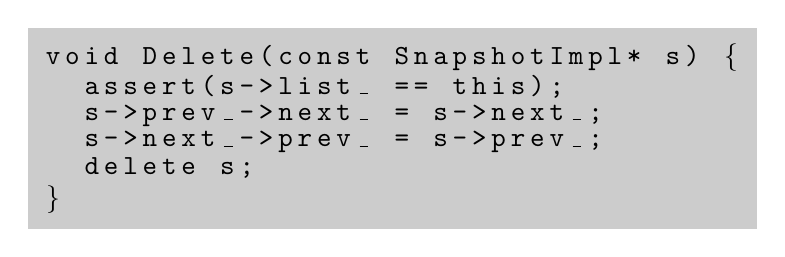
\begin{tikzpicture}
      \matrix {
v \& o \& i \& d \&   \& D \& e \& l \& e \& t \& e \& ( \& c \& o \& n \& s \& t \&   \& S \& n \& a \& p \& s \& h \& o \& t \& I \& m \& p \& l \& * \&   \& s \& ) \&   \& \{ \\
  \&   \& a \& s \& s \& e \& r \& t \& ( \& s \& - \& > \& l \& i \& s \& t \& \_ \&   \& = \& = \&   \& t \& h \& i \& s \& ) \& ; \\
  \&   \& s \& - \& > \& p \& r \& e \& v \& \_ \& - \& > \& n \& e \& x \& t \& \_ \&   \& = \&   \& s \& - \& > \& n \& e \& x \& t \& \_ \& ; \\
  \&   \& s \& - \& > \& n \& e \& x \& t \& \_ \& - \& > \& p \& r \& e \& v \& \_ \&   \& = \&   \& s \& - \& > \& p \& r \& e \& v \& \_ \& ; \\
  \&   \& d \& e \& l \& e \& t \& e \&   \& s \& ; \\
\} \\
      };
    \end{tikzpicture}
    \begin{tikzpicture}[remember picture,
                        overlay,
                        shift={(current page.south west)}]
      \node at (\paperwidth / 2, \paperheight * 12 / 16) [fill=yellow!50] {
Changes other linked list nodes through \texttt{s}
      };
      \visible<2> {
        \node [person] at (\paperwidth * 1 / 16, \paperheight / 6) {😱};
        \node [person] at (\paperwidth * 0.28125, \paperheight / 6) {😱};
        \node [person] at (\paperwidth * 0.71875, \paperheight / 6) {😱};
        \node [person] at (\paperwidth * 15 / 16, \paperheight / 6) {😱};
      }
    \end{tikzpicture}
  \end{frame}

  \begin{frame}
    \frametitle{Remaining Projects' Overall Results}
    \large
    \begin{tabular}{b{3.4cm} b{2.6cm} b{3.2cm}}
      \textbf{Project} & \textbf{Root Cause}
      & \textbf{Attribute} \\
      & & \\
      LLVM TableGen & \texttt{mutable} & Buffer / Caching \\
      Ninja & \texttt{mutable} & Unit Testing \\
      & & \\
      fish shell & \texttt{const\_cast} & Incorrect \\
      Mosh & \texttt{mutable} & Incorrect \\
      LLVM TableGen & \texttt{mutable} & Incorrect \\
      Tesseract & \texttt{mutable} & Incorrect \\
    \end{tabular}
  \end{frame}

  \begin{frame}
    \frametitle{LLVM Writes to a \texttt{mutable} Field}
    \centering
    \begin{tikzpicture}[remember picture,
                        overlay,
                        shift={(current page.south west)}]
      \matrix at (\paperwidth / 2, \paperheight * 6.5 / 10) {
v \& o \& i \& d \&   \& D \& F \& A \& P \& a \& c \& k \& e \& t \& i \& z \& e \& r \& E \& m \& i \& t \& t \& e \& r \& : \& : \& r \& u \& n \& ( \& |[black!50]|. \& |[black!50]|. \& |[black!50]|. \& ) \&   \& \{ \\
  \&   \& c \& o \& n \& s \& t \&   \& S \& t \& a \& t \& e \&   \& * \& N \& e \& w \& S \& t \& a \& t \& e \& ; \\
  \&   \& N \& e \& w \& S \& t \& a \& t \& e \&   \& = \&  \& D \& . \& n \& e \& w \& S \& t \& a \& t \& e \& ( \& ) \& ; \\
  \&   \& N \& e \& w \& S \& t \& a \& t \& e \& - \& > \& s \& t \& a \& t \& e \& I \& n \& f \& o \&   \& = \&   \& N \& e \& w \& S \& t \& a \& t \& e \& R \& e \& s \& o \& u \& r \& c \& e \& s \& ; \\
\} \\
      };
      \visible<2> {
        \node [person] at (\paperwidth * 1 / 16, \paperheight / 6) {😱};
        \node [person] at (\paperwidth * 0.28125, \paperheight / 6) {😱};
        \node [person] at (\paperwidth * 0.71875, \paperheight / 6) {😱};
        \node [person] at (\paperwidth * 15 / 16, \paperheight / 6) {😱};
      }
    \end{tikzpicture}
  \end{frame}

  \begin{frame}
    \frametitle{Tesseract Marks Header as Unreliable since Other Code Modifies}
    \centering
    \begin{tikzpicture}[remember picture,
                        overlay,
                        shift={(current page.south west)}]
      \matrix at (\paperwidth / 2, \paperheight * 5.5 / 10) {
c \& o \& n \& s \& t \&   \& c \& h \& a \& r \& * \&   \& S \& T \& R \& I \& N \& G \& : \& : \& s \& t \& r \& i \& n \& g \& ( \& ) \&   \& c \& o \& n \& s \& t \&   \& \{  \\
  \&   \& c \& o \& n \& s \& t \&   \& S \& T \& R \& I \& N \& G \& \_ \& H \& E \& A \& D \& E \& R \& * \&   \& h \& e \& a \& d \& e \& r \&   \& = \&   \& G \& e \& t \& H \& e \& a \& d \& e \& r \& ( \& ) \& ; \\
  \&   \& h \& e \& a \& d \& e \& r \& - \& > \& u \& s \& e \& d \& \_ \&   \& = \&   \& - \& 1 \& ; \\
  \&   \& r \& e \& t \& u \& r \& n \&   \& G \& e \& t \& C \& S \& t \& r \& ( \& ) \& ; \\
\} \\
      };
      \visible<2> {
        \node [person] at (\paperwidth * 1 / 16, \paperheight / 6) {😱};
        \node [person] at (\paperwidth * 0.28125, \paperheight / 6) {😱};
        \node [person] at (\paperwidth * 0.71875, \paperheight / 6) {😱};
        \node [person] at (\paperwidth * 15 / 16, \paperheight / 6) {😱};
      }
    \end{tikzpicture}
  \end{frame}

  \begin{frame}
    \frametitle{fish shell Removes \const{} then Writes}
    \centering
    \small
    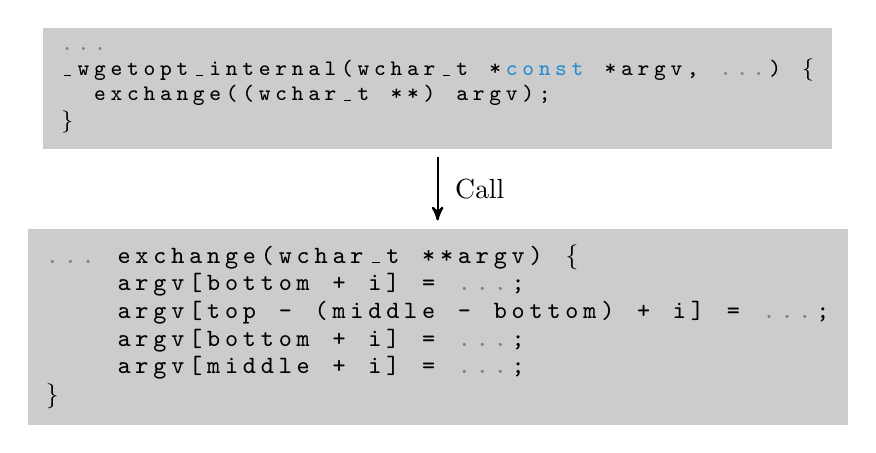
\begin{tikzpicture}

\footnotesize
      \matrix (wgetopt) {
|[black!50]|. \& |[black!50]|. \& |[black!50]|. \\

\_ \& w \& g \& e \& t \& o \& p \& t \& \_ \& i \& n \& t \& e \& r \& n \& a \& l \& ( \& w \& c \& h \& a \& r \& \_ \& t \&   \& * \& |[blue]|c \& |[blue]|o \& |[blue]|n \& |[blue]|s \& |[blue]|t \&   \& * \& a \& r \& g \& v \& , \&   \& |[black!50]|. \& |[black!50]|. \& |[black!50]|. \& ) \&   \& \{ \\
  \&   \& e \& x \& c \& h \& a \& n \& g \& e \& ( \& ( \& w \& c \& h \& a \& r \& \_ \& t \&   \& * \& * \& ) \&   \& a \& r \& g \& v \& ) \& ; \&   \&   \&   \&   \&   \&   \&   \&   \&   \&   \&   \&   \&   \&    \\
\} \&   \&   \&   \&   \&   \&   \&   \&   \&   \&   \&   \&   \&   \&   \&   \&   \&   \&   \&   \&   \&   \&   \&   \&   \&   \&   \&   \&   \&   \&   \&   \&   \&   \&   \&   \&   \&   \&   \&   \&   \&    \\
  };
\small
      \matrix (exchange) [scale=0.5, below=of wgetopt] {
|[black!50]|. \& |[black!50]|. \& |[black!50]|. \&   \& e \& x \& c \& h \& a \& n \& g \& e \& ( \& w \& c \& h \& a \& r \& \_ \& t \&   \& * \& * \& a \& r \& g \& v \& ) \&   \& \{ \\

  \&   \&   \&   \& a \& r \& g \& v \& \lbrack \& b \& o \& t \& t \& o \& m \&   \& + \&   \& i \& \rbrack \&   \& = \& \& |[black!50]|. \& |[black!50]|. \& |[black!50]|. \& ; \\

  \&   \&   \&   \& a \& r \& g \& v \& \lbrack \& t \& o \& p \&   \& - \&   \& ( \& m \& i \& d \& d \& l \& e \&   \& - \&   \& b \& o \& t \& t \& o \& m \& ) \&   \& + \&   \& i \& \rbrack \&   \& = \& \& |[black!50]|. \& |[black!50]|. \& |[black!50]|. \& ; \\

  \&   \&   \&   \& a \& r \& g \& v \& \lbrack \& b \& o \& t \& t \& o \& m \&   \& + \&   \& i \& \rbrack \&   \& = \&   \&  |[black!50]|. \& |[black!50]|. \& |[black!50]|. \& ; \\

  \&   \&   \&   \& a \& r \& g \& v \& \lbrack \& m \& i \& d \& d \& l \& e \&   \& + \&   \& i \& \rbrack \&   \& = \&   \&  |[black!50]|.\& |[black!50]|. \& |[black!50]|. \& ;   \\

        \} \\
      };

      \draw [arrow] (wgetopt) -- node [right, xshift=1mm] {\normalsize Call} (exchange);
    \end{tikzpicture}

    \begin{tikzpicture}[remember picture,
                        overlay,
                        shift={(current page.south west)}]
      \node at (\paperwidth / 2, \paperheight * 13.5 / 16) [fill=yellow!50] {
Declares function won't change order of strings in array
      };
      \node at (\paperwidth * 8.1 / 10, \paperheight * 5.65 / 10) [fill=yellow!50] {
Changes order of strings
      };
      \visible<2> {
      \node (c) at (\paperwidth * 6.6 / 10, \paperheight / 9)
             [inner sep=0, circle, minimum size=6mm, scale=0.7,
             fill=green]
            {$\checkmark$};
      \node [node distance=0, green, right=of c] {\bfseries Fixed by developers};
      }
    \end{tikzpicture}
  \end{frame}

  \begin{frame}
    \frametitle{Mosh Writes Directly Through \const{}}
    \centering
    \small
    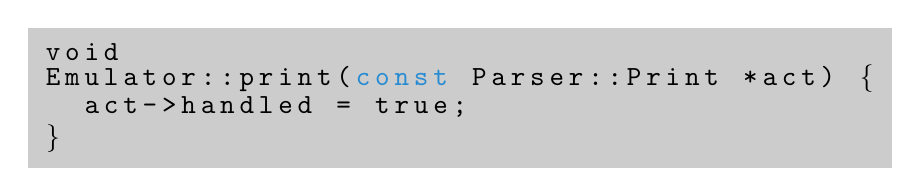
\begin{tikzpicture}
      \matrix  {
v \& o \& i \& d \\

E \& m \& u \& l \& a \& t \& o \& r \& : \& : \& p \& r \& i \& n \& t \& ( \& |[blue]|c \& |[blue]|o \& |[blue]|n \& |[blue]|s \& |[blue]|t \&   \& P \& a \& r \& s \& e \& r \& : \& : \& P \& r \& i \& n \& t \&   \& * \& a \& c \& t \& ) \&   \& \{ \\
  \&   \& a \& c \& t \& - \& > \& h \& a \& n \& d \& l \& e \& d \&   \& = \&   \& t \& r \& u \& e \& ; \\

\} \\
      };
    \end{tikzpicture}
    \begin{tikzpicture}[remember picture,
                        overlay,
                        shift={(current page.south west)}]
      \visible<2> {
      \node (c) at (\paperwidth * 6.6 / 10, \paperheight / 9)
             [inner sep=0, circle, minimum size=6mm, scale=0.7,
             fill=green]
            {$\checkmark$};
      \node [node distance=0, green, right=of c] {\bfseries Fixed by developers};
      }
    \end{tikzpicture}
  \end{frame}

  \begin{frame}
    \frametitle{Answers to Research Questions}
    \large
    \begin{enumerate}
      \setlength\itemsep{0.5em}
      \item Developers write-through-\const{}
      \item Shallow and deep bitwise violated equally
      \item Around half of writes-through-\const{}

            are not logically immutable

            \vspace{2em}
            They appear to be undesirable

since developers fix them

            % they are fixed by developers
    \end{enumerate}
  \end{frame}

  \begin{frame}
    \frametitle{Try It Out}

    \begin{tikzpicture}[remember picture,
                        overlay,
                        shift={(current page.south west)}]
      \node at (\paperwidth / 3, \paperheight / 2) {
\includegraphics[scale=0.1]{aec-badge-ecoop}};
      \node [inner sep=0, anchor=east] (github) at (\paperwidth * 2/ 3, \paperheight / 2) {
\includegraphics[scale=0.15]{github-logo}};
      \node [inner sep=0, node distance=1mm, right=of github.south east, anchor=south west] {\Large \texttt{/eyolfson/}};
      \node (art) [node distance=2mm, below=of github.south east, xshift=2mm] {\small \texttt{research-2016-ecoop-artifact}};
      \node [inner sep=0, node distance=0, below=of art] {\small \texttt{research-2016-ecoop-paper}};
      \node [node distance=8mm, above=of github.south east] {\Large \texttt{https://eyl.io/}};
    \end{tikzpicture}

  \end{frame}
\end{document}
